%
% ---------- chapter 5 ----------
%

\section{Empirical Study}
%
To assess the evolutionary algorithm proposed in this paper, two separated
evaluation experiments are made for the efficiency of parallel evolutionary
algorithm and the validity of evolutionary algorithm in project management
problem. The purpose of the experiment is to answer the following two questions:


\textbf{RQ1}: Does the evolutionary algorithm effectively optimize project
management problem, and get an optimized answer?

\textbf{RQ2}: Is the parallel evolutionary algorithm able to improve the
efficiency in the project management problem?


\subsection{Experimental Data}
%
The experimental data evaluated in this paper are real industrial project
management plans.


There are three software project plannings, which are named
as \emph{A-Input}, \emph{B-DBUpgrade} and \emph{C-SmartPrice}, where
\emph{A-Input} is a simulated medium-scale project planning. \emph{B-DBUpgrade}
is the project plan of the Oracle database upgrade. The goal of
\emph{B-DBUpgrade} is to upgrade the Oracle database from the \emph{9g} version
to the \emph{10g} version, which is Oracle's non-public version of the project
planning. \emph{C-SmartPrice} is a medium-sized project planning about supply
chain upgrade, and like B,it is a non-public of the internal project planning
\cite{ren}. The related statistics is shown in Table \ref{table:statis}.

\begin{table}
  \caption{Statistics of Three Projects}
  \label{table:statis}
  \begin{center}
  \begin{tabular}{lccc}
    \hline
      & \emph{ A-Input } & \emph{ B-DBUpgrade } & \emph{ C-SmartPrice } \\
    \hline
    number of \emph{work packages} & 33 & 106 & 74 \\
    number of \emph{resources}     & 4  & 8   & 14 \\
    number of \emph{dependencies}  & 35 & 105 & 73 \\
    \hline
  \end{tabular}
  \end{center}
\end{table}


\subsection{Validastion Experiment for Algorithm}
%
In order to answer \textbf{RQ1}, this section designs the validation experiment for 
evolutionary algorithm. The basic configuration used in the effectiveness 
evaluation experiment is that the number of individuals is 100 and the number 
of iterations is 100. For each computational 
process of the evolutionary algorithm, we count the fitness for each 
generations of the population, and then plot the discrete fitness results 
into a box graph.


Each generation of the graph shows the five eigenvalues of all individual 
fitness in the population: the minimum, the next quartile, the median, the 
upper quartile and the maximum. We draw the box graphs which is corresponding 
to the calculation results of the values for each generation of the three 
project inputted, which show in Figure 12, Figure 13 and Figure 14. From the 
trend of three projects, it can be seen that the population is more 
diversified when the population is initialized, and the span of the box is 
larger as the number of iterations increases. The population evolves toward 
the better result, At the same time the overall suitability begins to 
decrease, and finally the approximation converges to a superior result.


Through the above analysis results of experimental data, we can accurately 
answer \textbf{RQ1}. In the project management problems, the evolutionary algorithm does 
have a good space of optimization and improvement.

\begin{figure}[ht]
  \centering
  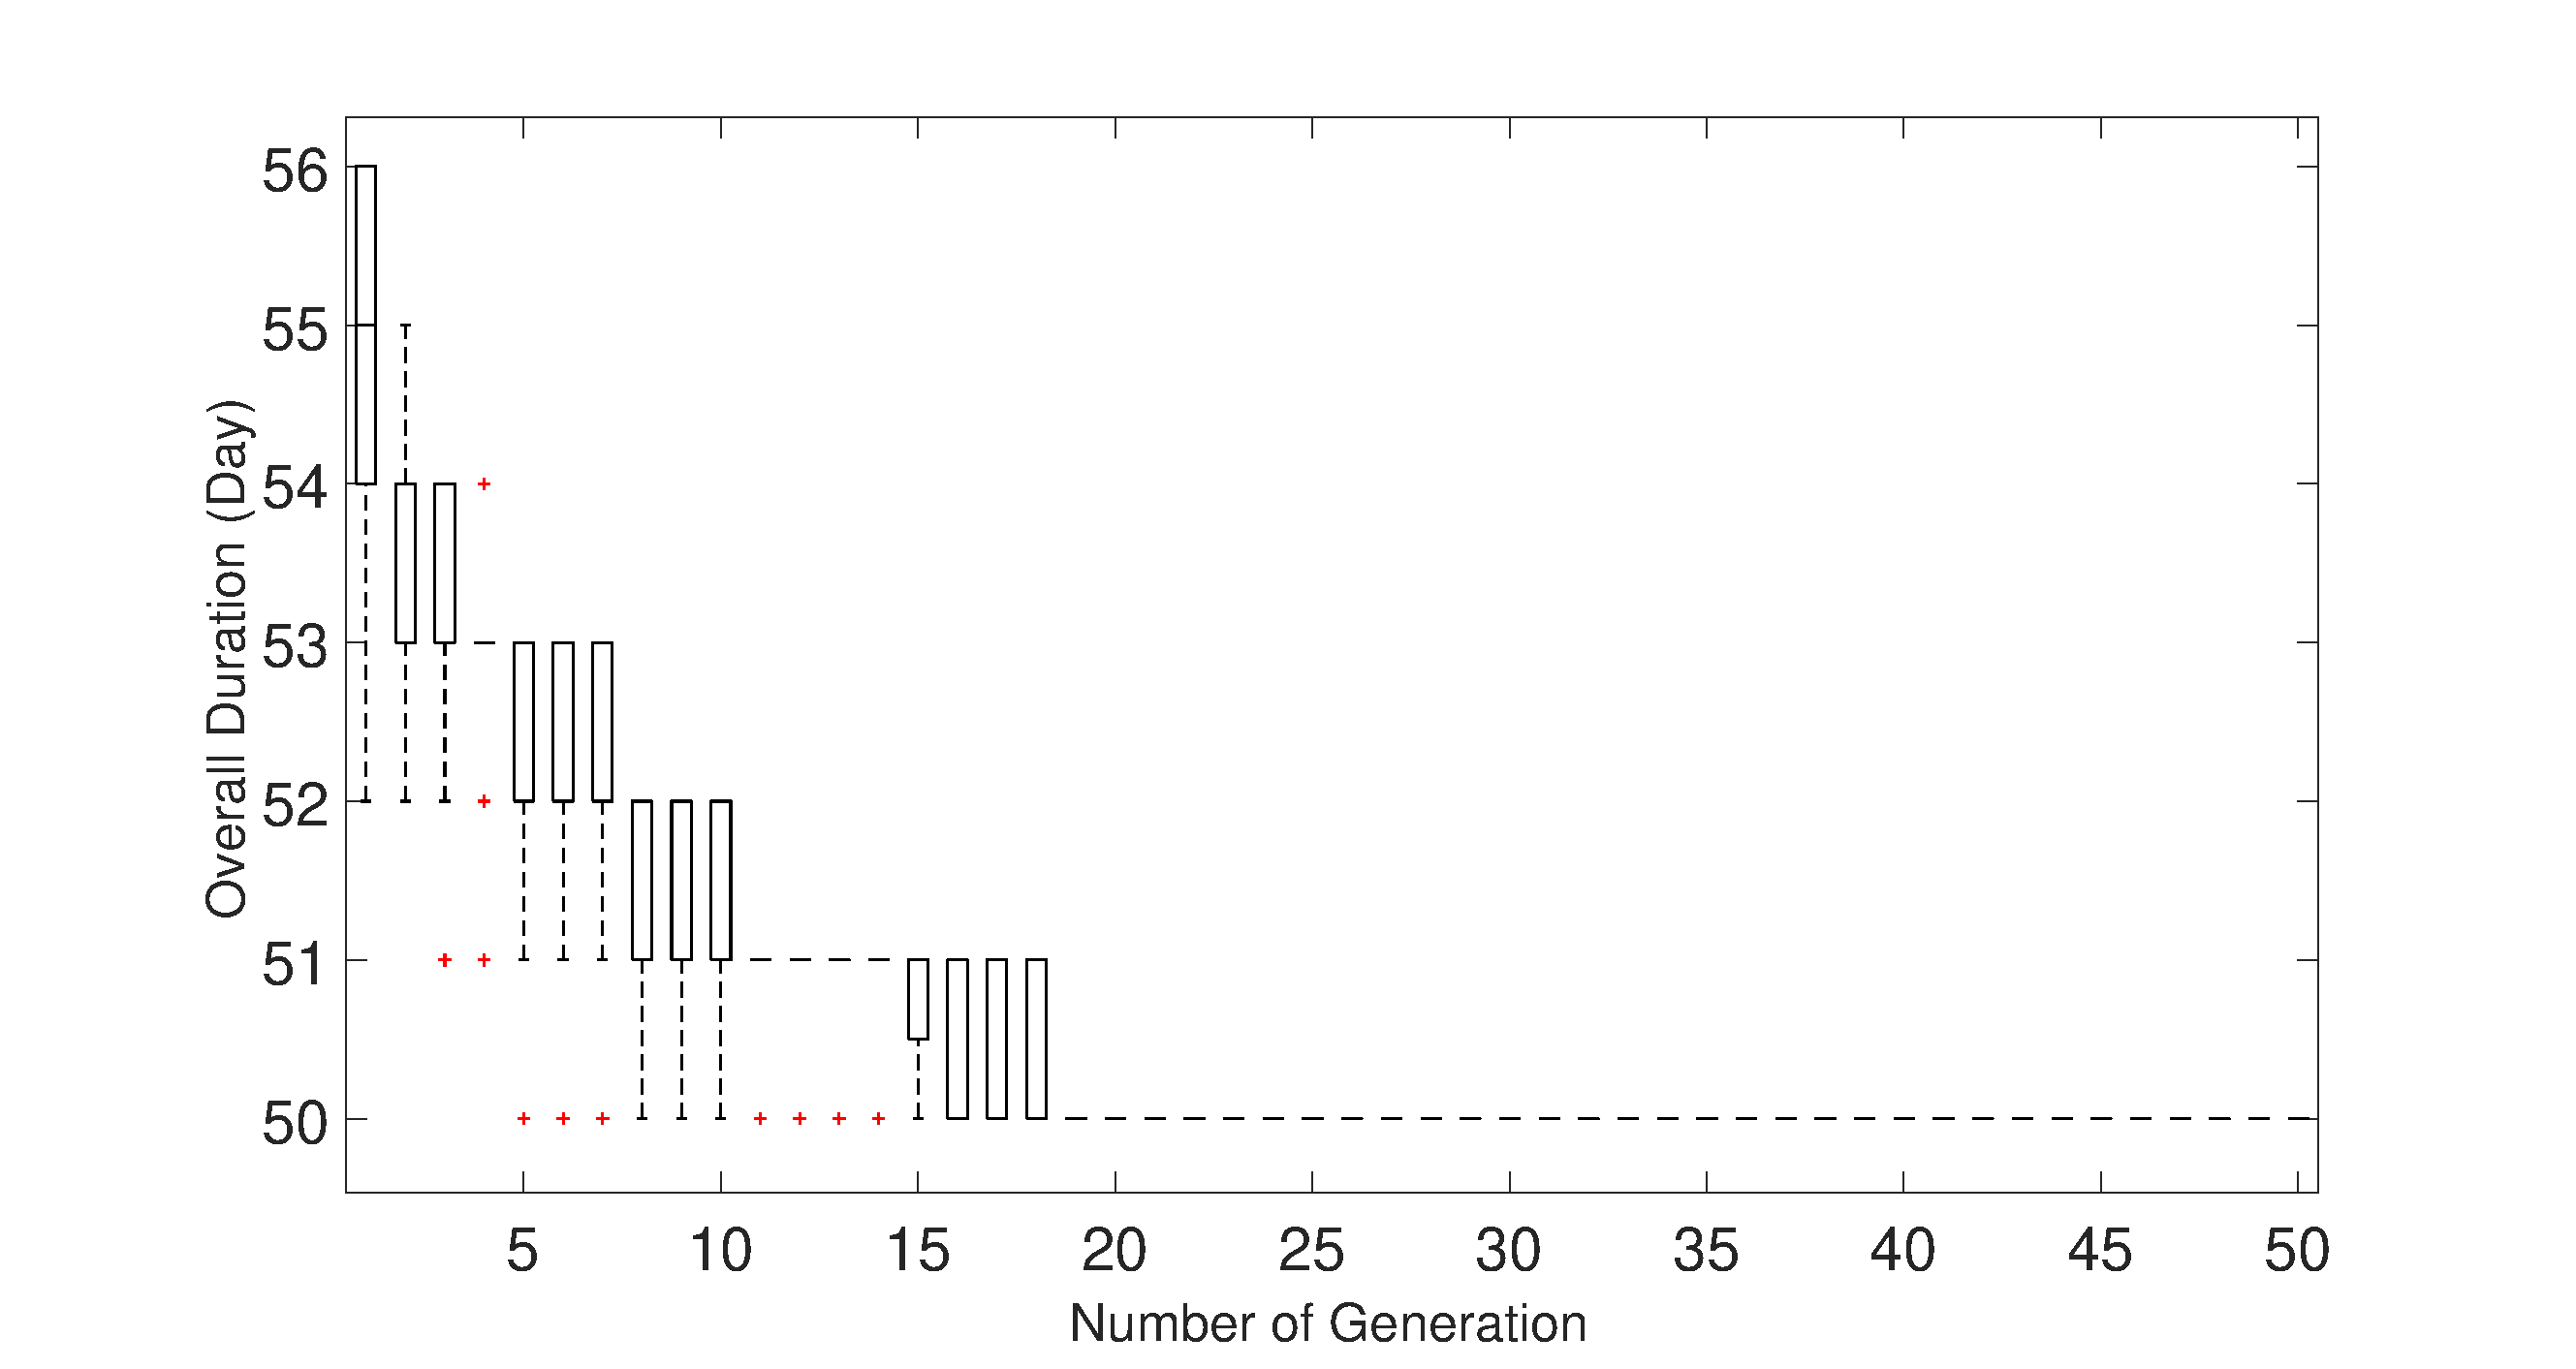
\includegraphics[width=\textwidth]{figures/fig_pa1.eps}
  \caption{figure 11}
  \label{fig:label}
\end{figure}


%figure12
%figure13
%figure14





\subsection{Evaluation Experimeent for Algorithm Efficiency}
%
In order to answer \textbf{RQ2}, this section achieves the efficiency comparison
test between the parallel evolution algorithm and serial evolution
algorithm. The hardware environment of this experiment is as follows: the
runtime environment that execute the serial evolution algorithm is the Intel i7
series central processing unit (CPU). The runtime environment of the parallel
evolution algorithm is the NVidia GeForce series graphics processing unit (GPU
). CPU and GPU detailed configuration comparison see Table 6.1. The software
environment of this experiment is: Window 7 Ultimate Service Pack 1, Microsoft
Visual Studio 2012 C++ Compiler, CUDA 7.0.28 Runtime compilation
environment. The specific hardware configuration is shown in Table 2.

%table 2

This experiment uses the above three items as input to evaluate the performance
comparison of the parallel evolutionary algorithm and the serial evolution
algorithm. The specific work about encoding has actually completed two versions
of the project management algorithm, the serial version is written in C++
language and parallel version is written using CUDA C++ language. It is used to
verify the difference between the parallel evolutionary algorithm and the serial
evolution algorithm in project management problem by the code design experiment
of the two versions.


pThe initial configuration of the two versions is the same. The number of
populations is 1000, and the number of iterations is 100. Each iteration process
includes crossover, mutation and selection.  Each time the iteration process
sets the timer at the beginning of an evolutionary algorithm to counts 100
iterations, and then stops the timer after 100 iterations. This allows us to
count the total computational time of the project problem in the serial CPU
environment and the parallel GPU environment, using this time as the evaluation
criteria.

%figure 9
%figure10
%figure11

The 10 time-consuming charts for Project A, Project B, and Project C are 
shown in Figures 9, 10 and 11. It can be seen from the figures that the time-
consuming on the CPU algorithm is roughly twice as long as the GPU algorithm. 
At the same time, the advantage of using the GPU algorithm in the calculation 
of project management problems is that we can make better use of system 
resources. So it can be a good answer to \textbf{RQ2} that parallel evolution 
algorithm can effectively improve the efficiency of computing in the project 
management problems.
